\documentclass{article}

\usepackage[utf8]{inputenc}
\usepackage{mdwlist}
\usepackage[inner=3cm,outer=4cm]{geometry}
\usepackage{mathtools}

\usepackage{Sweave}
\begin{document}
\Sconcordance{concordance:HW07PLS206F14.tex:HW07PLS206F14.Rnw:%
1 7 1 1 0 19 1 1 10 9 0 5 1 1 6 8 0 1 2 3 1 1 2 1 0 7 1 4 0 1 2 9 1 1 2 %
1 0 1 1 35 0 1 1 24 0 1 1 20 0 1 2 2 1 1 2 1 0 1 1 19 0 1 2 2 1 1 2 1 0 %
1 1 17 0 1 1 12 0 1 2 2 1 1 2 1 0 1 1 16 0 1 1 11 0 1 1 6 0 1 2 6 1 1 2 %
1 0 1 1 13 0 1 2 4 1 1 2 1 0 1 1 4 0 1 2 4 1 1 2 31 0 1 2 6 1 1 5 1 0 2 %
1 24 0 1 3 3 1 1 3 7 0 1 1 5 0 1 1 5 0 2 1 1 6 8 0 1 2 7 1}


\title{Homework 07. GLMs. PLS206 Fall 2014}
\author{Emilio A. Laca}
\maketitle

\section{Data}

This exercise uses simulated data. Thus, we know the true model and whether the assumptions are met. The data simulate the number of individuals of a relatively rare mammal observed in a series of locations in East Africa. Locations were selected haphazardly. Variables measured at each location were:

\begin{description*}
  \item[nrrm] number of individuals of the relatively rare mammal seen.
  \item[river] distance to the nearest river in km.
  \item[tveg] vegetation type (sg: short grass, tg: tall grass, sh: shrubs, wl: woodland, svn: savanna )
  \item[road] distance to nearest road in km.
  \item[cover] visual cover; proportion of a vertical surface visible from 20 m.
\end{description*}

The data simulation code is presented for completeness, but for the analysis we use a preset simulation that remains constant across compilations of this document.
\begin{Schunk}
\begin{Sinput}
> dsim <- data.frame(river = round(runif(100, min=0.5, max=15),1),
+                  tveg = rep(c("sg","tg","sh","wl","svn"),each=20),
+                  road = round(rchisq(100, 6),1),
+                  cover = c(
+                    rbeta(20,2,10),
+                    rbeta(20,4,8),
+                    rbeta(20,10,3),
+                    rbeta(20,8,4),
+                    rbeta(20,6,6)))
> beta0 <- 0.05
> bRiver <- -0.09
> bRoad <- 0.04
> bRiverRoad <- 0.01
> bCover <- 2
> dsim$nrrm <- rpois(100,
+                  exp(beta0 +
+                      bRiver*dsim$river +
+                      bRoad*dsim$road +
+                      bRiverRoad*dsim$river*dsim$road +
+                      bCover*dsim$cover))
\end{Sinput}
\end{Schunk}

\section{Data exploration}
We start with the hypothesis that the species will be more abundant in grassland areas with good cover close to rivers and far from roads. We plot the data against each predictor.

\begin{Schunk}
\begin{Sinput}
> d1 <- read.csv("../Examples/dataHW07F14.txt", header=TRUE)
> library(car)
> library(ggplot2)
> par(mfrow=c(3,1))
> scatterplot(nrrm ~ river | tveg, data=d1)
> scatterplot(nrrm ~ road | tveg, data=d1)
> scatterplot(nrrm ~ cover | tveg, data=d1)
> pairs(d1)
\end{Sinput}
\end{Schunk}
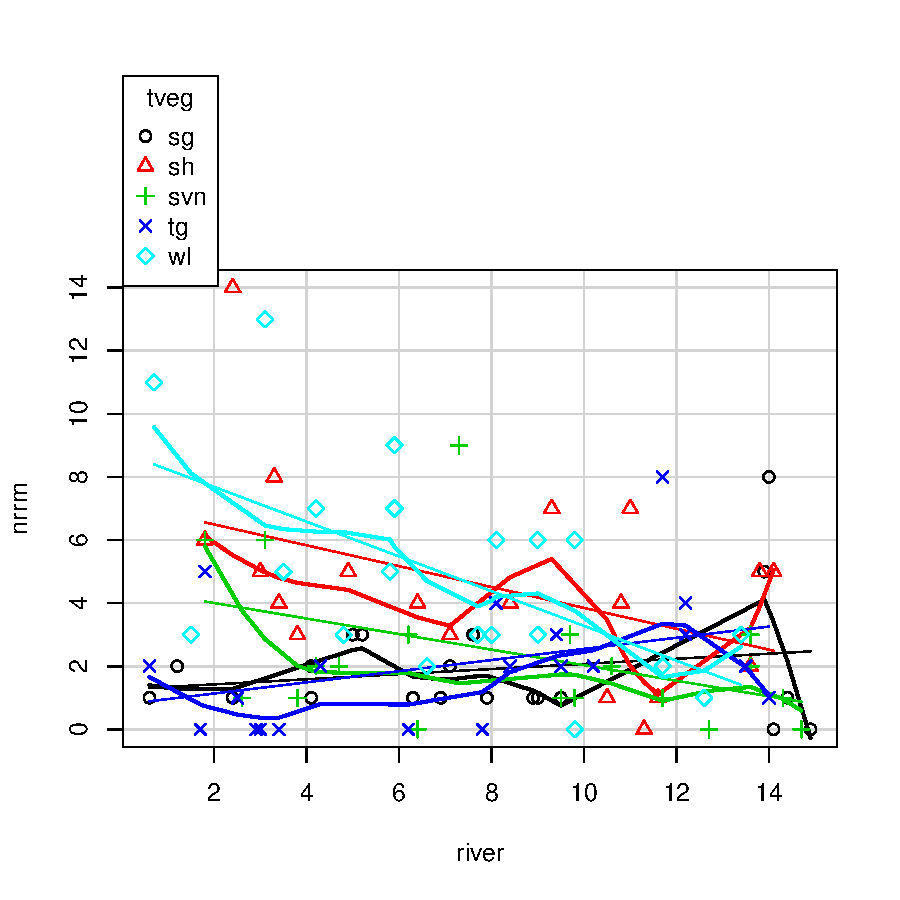
\includegraphics{HW07PLS206F14-explore}

There are clear trends in the plots for cover and roads, but the effect of distance to rivers appears weak. This may be a result of the variability that masks the effects. A model will "clean up" the variability and make it easier to see patterns. Cover is clearly related to vegetation type. This collinearity may make it difficult to pick the correct "causal" factor.


\section{Modeling}
\subsection{Why use Poisson?}
The number of individuals counted is a positive discrete variable. There is no limit to the potential number of individuals found. We start with a distribution that accommodates both properties, the Poisson distribution. We must take into account the fact that there are 100 observations, thus, we should not entertain models with more than 15 degrees of freedom.

\subsection{Select a model starting with tveg plus main effects and second order interactions for the other predictors.}

\begin{Schunk}
\begin{Sinput}
> m1 <- glm(nrrm ~ tveg + (cover+river+road)^2, family="poisson", data=d1)
> summary(m1)
\end{Sinput}
\begin{Soutput}
Call:
glm(formula = nrrm ~ tveg + (cover + river + road)^2, family = "poisson", 
    data = d1)

Deviance Residuals: 
    Min       1Q   Median       3Q      Max  
-2.9353  -0.7593  -0.2266   0.5935   2.1243  

Coefficients:
             Estimate Std. Error z value Pr(>|z|)   
(Intercept) -0.177697   0.473784  -0.375  0.70762   
tvegsh       0.249585   0.341043   0.732  0.46427   
tvegsvn     -0.081379   0.260997  -0.312  0.75519   
tvegtg      -0.119652   0.233822  -0.512  0.60885   
tvegwl       0.187744   0.339702   0.553  0.58049   
cover        2.263827   0.731576   3.094  0.00197 **
river       -0.035029   0.050847  -0.689  0.49089   
road         0.057530   0.041790   1.377  0.16862   
cover:river -0.104230   0.063010  -1.654  0.09809 . 
cover:road  -0.019695   0.062959  -0.313  0.75441   
river:road   0.007551   0.003638   2.075  0.03796 * 
---
Signif. codes:  0 ‘***’ 0.001 ‘**’ 0.01 ‘*’ 0.05 ‘.’ 0.1 ‘ ’ 1

(Dispersion parameter for poisson family taken to be 1)

    Null deviance: 247.67  on 99  degrees of freedom
Residual deviance: 113.03  on 89  degrees of freedom
AIC: 391.06

Number of Fisher Scoring iterations: 5
\end{Soutput}
\begin{Sinput}
> anova(m1, test="Chisq")
\end{Sinput}
\begin{Soutput}
Analysis of Deviance Table

Model: poisson, link: log

Response: nrrm

Terms added sequentially (first to last)


            Df Deviance Resid. Df Resid. Dev  Pr(>Chi)    
NULL                           99     247.67              
tveg         4   50.740        95     196.93 2.530e-10 ***
cover        1    6.132        94     190.80  0.013273 *  
river        1    9.329        93     181.47  0.002255 ** 
road         1   58.590        92     122.88 1.942e-14 ***
cover:river  1    5.338        91     117.54  0.020865 *  
cover:road   1    0.116        90     117.42  0.733174    
river:road   1    4.396        89     113.03  0.036018 *  
---
Signif. codes:  0 ‘***’ 0.001 ‘**’ 0.01 ‘*’ 0.05 ‘.’ 0.1 ‘ ’ 1
\end{Soutput}
\begin{Sinput}
> Anova(m1, test="Wald", type=3)
\end{Sinput}
\begin{Soutput}
Analysis of Deviance Table (Type III tests)

Response: nrrm
            Df  Chisq Pr(>Chisq)   
(Intercept)  1 0.1407   0.707617   
tveg         4 2.7900   0.593566   
cover        1 9.5756   0.001972 **
river        1 0.4746   0.490889   
road         1 1.8952   0.168616   
cover:river  1 2.7363   0.098090 . 
cover:road   1 0.0979   0.754411   
river:road   1 4.3067   0.037962 * 
Residuals   89                     
---
Signif. codes:  0 ‘***’ 0.001 ‘**’ 0.01 ‘*’ 0.05 ‘.’ 0.1 ‘ ’ 1
\end{Soutput}
\end{Schunk}

The type \verb!Anova()! tests show that the least significant effect is the interaction between cover and road. We can eliminate that term and repeat the test to determine who can be eliminated next

\begin{Schunk}
\begin{Sinput}
> m2 <- glm(nrrm ~ tveg + (cover+river+road)^2 - cover:road, family="poisson", data=d1)
> Anova(m2, test="Wald", type=3)
\end{Sinput}
\begin{Soutput}
Analysis of Deviance Table (Type III tests)

Response: nrrm
            Df   Chisq Pr(>Chisq)    
(Intercept)  1  0.0653  0.7983718    
tveg         4  2.8500  0.5832349    
cover        1 13.4297  0.0002477 ***
river        1  0.4790  0.4888741    
road         1  2.9314  0.0868736 .  
cover:river  1  2.7254  0.0987631 .  
river:road   1  4.3257  0.0375409 *  
Residuals   90                       
---
Signif. codes:  0 ‘***’ 0.001 ‘**’ 0.01 ‘*’ 0.05 ‘.’ 0.1 ‘ ’ 1
\end{Soutput}
\end{Schunk}

Now, tveg is the variable that is least significant when entered last, so it is removed next. We drop model terms with the restriction that if an interaction is significant, the main effects involved must be kept in the model.

\begin{Schunk}
\begin{Sinput}
> m3 <- glm(nrrm~cover+river+road+cover:river+road:river, family="poisson", data=d1)
> Anova(m3, test="Wald", type=3)
\end{Sinput}
\begin{Soutput}
Analysis of Deviance Table (Type III tests)

Response: nrrm
            Df   Chisq Pr(>Chisq)    
(Intercept)  1  0.9362    0.33326    
cover        1 33.1866  8.373e-09 ***
river        1  0.2296    0.63179    
road         1  6.1793    0.01293 *  
cover:river  1  2.8593    0.09085 .  
river:road   1  3.2902    0.06969 .  
Residuals   94                       
---
Signif. codes:  0 ‘***’ 0.001 ‘**’ 0.01 ‘*’ 0.05 ‘.’ 0.1 ‘ ’ 1
\end{Soutput}
\begin{Sinput}
> anova(m1,m3, test="Chisq")
\end{Sinput}
\begin{Soutput}
Analysis of Deviance Table

Model 1: nrrm ~ tveg + (cover + river + road)^2
Model 2: nrrm ~ cover + river + road + cover:river + road:river
  Resid. Df Resid. Dev Df Deviance Pr(>Chi)
1        89     113.03                     
2        94     116.00 -5  -2.9695   0.7047
\end{Soutput}
\end{Schunk}

The \verb!anova()! test shows that in spite of the terms dropped the current model is not significantly worse than the initial full model. The Type III tests suggest that the next candidate for deletion is cover:river.

\begin{Schunk}
\begin{Sinput}
> m4 <- glm(nrrm~cover+river+road+road:river, family="poisson", data=d1)
> Anova(m4, test="Wald", type=3)
\end{Sinput}
\begin{Soutput}
Analysis of Deviance Table (Type III tests)

Response: nrrm
            Df   Chisq Pr(>Chisq)    
(Intercept)  1  0.0543   0.815786    
cover        1 65.0135  7.439e-16 ***
river        1 10.5781   0.001144 ** 
road         1  4.4645   0.034607 *  
river:road   1  6.2043   0.012744 *  
Residuals   95                       
---
Signif. codes:  0 ‘***’ 0.001 ‘**’ 0.01 ‘*’ 0.05 ‘.’ 0.1 ‘ ’ 1
\end{Soutput}
\begin{Sinput}
> anova(m1,m4, test="Chisq")
\end{Sinput}
\begin{Soutput}
Analysis of Deviance Table

Model 1: nrrm ~ tveg + (cover + river + road)^2
Model 2: nrrm ~ cover + river + road + road:river
  Resid. Df Resid. Dev Df Deviance Pr(>Chi)
1        89     113.03                     
2        95     118.82 -6  -5.7891   0.4472
\end{Soutput}
\begin{Sinput}
> AIC(m4)
\end{Sinput}
\begin{Soutput}
[1] 384.8451
\end{Soutput}
\end{Schunk}

This final model has only significant terms, it has the lowest AIC, and it is not significantly worse than the full model. This is a good candidate for final model and we keep it. There may be one other model that has similar properties, and that would also be a good choice.

\subsection{Test for overdispersion}
This model include all the seemingly important factors, but it may have a problem of overdispersion. Overdispersion refers to the violation of the implicit assumption that the mean is equal to the variance for Poisson distributed data. If the assumption is true, then the residual deviance should have a $\chi^2$ distribution with n-p = 95 df. The value of 118.82 with 95 df has a probability of 0.05, which is suggestive of overdispersion.

One way to test for overdispersion is to fit a model using the quasipoisson family, which has one additional parameter to allow for a variance that is greater (by a constant factor) than the mean. Technically, the model development should be repeated with the new approach, but here we just test for overdispersion. The package AER has a function \verb!dispersiontest()! that performs a test of significance of overdispersion.
\begin{Schunk}
\begin{Sinput}
> library(AER)
> dispersiontest(m4, trafo=1)
\end{Sinput}
\begin{Soutput}
	Overdispersion test

data:  m4
z = 0.2895, p-value = 0.3861
alternative hypothesis: true alpha is greater than 0
sample estimates:
     alpha 
0.03754761 
\end{Soutput}
\end{Schunk}

The test indicates that there is no significant overdispersion, which is consistent with the fact that data were actually simulated from a Poisson distribution.

\subsection{Inspection of residuals}

\begin{Schunk}
\begin{Sinput}
> par(mfrow=c(2,2))
> plot(m4)
\end{Sinput}
\end{Schunk}
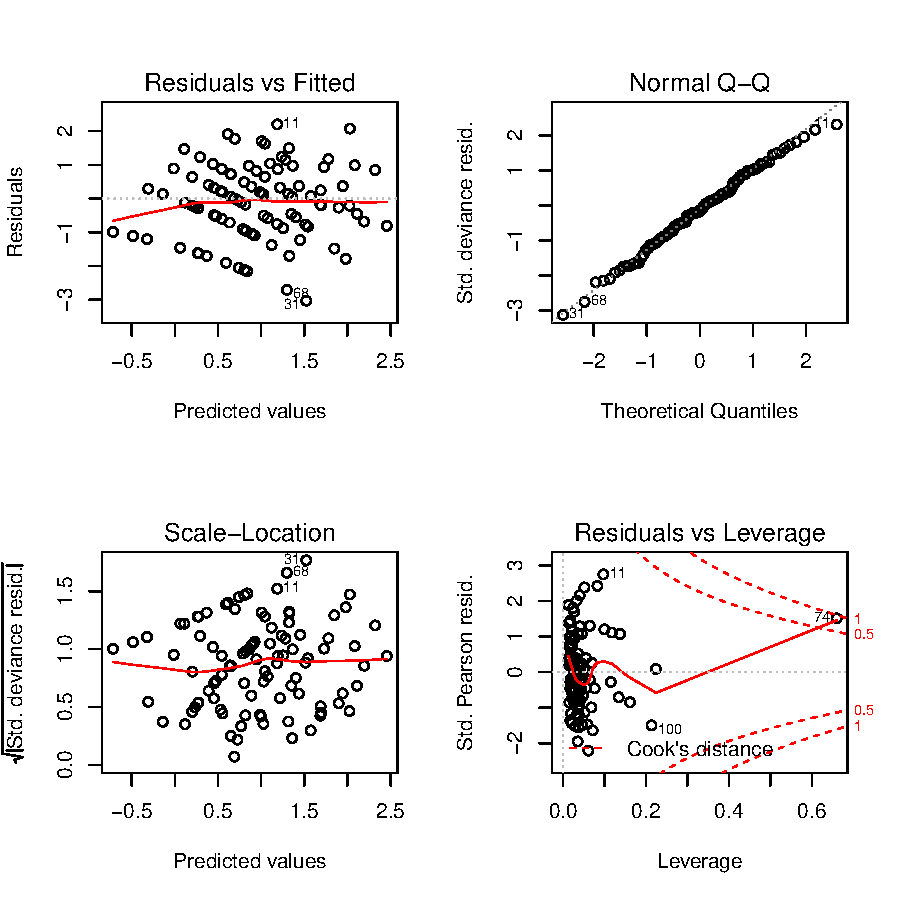
\includegraphics{HW07PLS206F14-008}

The plot of response or raw residuals show no pattern deviating from a flat overall trend. The normal Q-Q plot exhibits a strong agreement with the straight line representing normality of the standardized deviance residuals. This means that the assumption of normality for large sample size appears to be correct, and that the tests that are based on asymptotic normality are expected to give good estimates of the true probabilities.The graph of standardized deviance residuals is also flat and shows no deviation of expectation, with the potential appearance of low variance for low predicted values. Unlike the raw residuals whose variance is supposed to change with the mean, the standardized deviation residuals are expected to have constant variance. The appearance of low variance in the left is most likely just an inaccurate visual impression due to the fact that there are few observations in that range. Finally, the leverage plot shows that observation 74 has high leverage and it is influential. This observation should be checked for errors or unusual circumstances (if it were real). Given that the observation comes from a known model and distribution via simulation, we can simply use it to understand that outliers happen. Even when everything is OK.

\subsection{Effect of cover}

\begin{Schunk}
\begin{Sinput}
> summary(m4)
\end{Sinput}
\begin{Soutput}
Call:
glm(formula = nrrm ~ cover + river + road + road:river, family = "poisson", 
    data = d1)

Deviance Residuals: 
    Min       1Q   Median       3Q      Max  
-3.0280  -0.8414  -0.1481   0.6661   2.2005  

Coefficients:
            Estimate Std. Error z value Pr(>|z|)    
(Intercept)  0.06168    0.26477   0.233  0.81579    
cover        1.94877    0.24169   8.063 7.44e-16 ***
river       -0.09361    0.02878  -3.252  0.00114 ** 
road         0.05002    0.02367   2.113  0.03461 *  
river:road   0.00802    0.00322   2.491  0.01274 *  
---
Signif. codes:  0 ‘***’ 0.001 ‘**’ 0.01 ‘*’ 0.05 ‘.’ 0.1 ‘ ’ 1

(Dispersion parameter for poisson family taken to be 1)

    Null deviance: 247.67  on 99  degrees of freedom
Residual deviance: 118.82  on 95  degrees of freedom
AIC: 384.85

Number of Fisher Scoring iterations: 5
\end{Soutput}
\end{Schunk}

As cover increases by one unit, the log of the expected number or abundance of the rare mammal is expected to increase by 1.95 units. Because of the link function, the predictors are no longer linearly related to the mean response. Thus, in terms of difference in the expected number of individuals of the rare mammal, the effect of a unit increase in cover depends on specific range where that increment takes place. Therefore, it is easiest to comprehend and communicate the effects of predictors by using graphical representations. Note that when using graphics, error or confidence bars will be asymmetric. Confidence or bar extremes should be calculated in the link dimension and "back-transformed" in the last step prior to drawing the graphs.

\subsection{Tabular and graphical interpretation of effects}

First we calculate a table of values to represent the effects of predictors.

\begin{Schunk}
\begin{Sinput}
> t.data <- expand.grid(cover=c(0.25,0.75), river=c(1,5),road=c(2,20))
> t.data$nrrm <- predict(m4,newdata=t.data, type="response")
> print(xtable(t.data))
\end{Sinput}
% latex table generated in R 3.1.2 by xtable 1.7-4 package
% Tue Dec  9 20:23:37 2014
\begin{table}[ht]
\centering
\begin{tabular}{rrrrr}
  \hline
 & cover & river & road & nrrm \\ 
  \hline
1 & 0.25 & 1.00 & 2.00 & 1.77 \\ 
  2 & 0.75 & 1.00 & 2.00 & 4.69 \\ 
  3 & 0.25 & 5.00 & 2.00 & 1.30 \\ 
  4 & 0.75 & 5.00 & 2.00 & 3.44 \\ 
  5 & 0.25 & 1.00 & 20.00 & 5.03 \\ 
  6 & 0.75 & 1.00 & 20.00 & 13.34 \\ 
  7 & 0.25 & 5.00 & 20.00 & 6.57 \\ 
  8 & 0.75 & 5.00 & 20.00 & 17.42 \\ 
   \hline
\end{tabular}
\end{table}\begin{Sinput}
> 
\end{Sinput}
\end{Schunk}

Mammal abundance increases exponentially with increasing cover at all distances from rivers and roads. The abundance is inversely proportional to distance from roads. The positive interaction between river and road is shown by the fact that at short distances to roads (2) the highest abundance is near rivers, whereas the reverse is true for long distances from rivers. This, of course has no factual value because the data were simulated by your professor to show some sort of plausible and sensible distribution of a mammal that likes to have lots of cover and be away from roads.

Finally, we use more prediction points to make a smoother version of the response of mammal abundance to changes in predictor values.
\begin{Schunk}
\begin{Sinput}
> # Predictions for various levels of cover and distance to river at average level of road
> mean(d1$road)
\end{Sinput}
\begin{Soutput}
[1] 6.172
\end{Soutput}
\begin{Sinput}
> range(d1$river)
\end{Sinput}
\begin{Soutput}
[1]  0.6 14.9
\end{Soutput}
\begin{Sinput}
> range(d1$cover)
\end{Sinput}
\begin{Soutput}
[1] 0.03181025 0.93092131
\end{Soutput}
\begin{Sinput}
> p.data <- expand.grid(cover=seq(0.04,0.94,by=0.05), river=c(0,5,10,15),road=c(2,20))
> p.data$nrrm <- predict(m4,newdata=p.data, type="response")
> ggplot(p.data, aes(x = cover, y = nrrm, colour = factor(river))) +
+   geom_point() +
+   geom_line() +
+   facet_wrap(~road) +
+   labs(x = "Cover", y = "Predicted number of rare mammal")
\end{Sinput}
\end{Schunk}
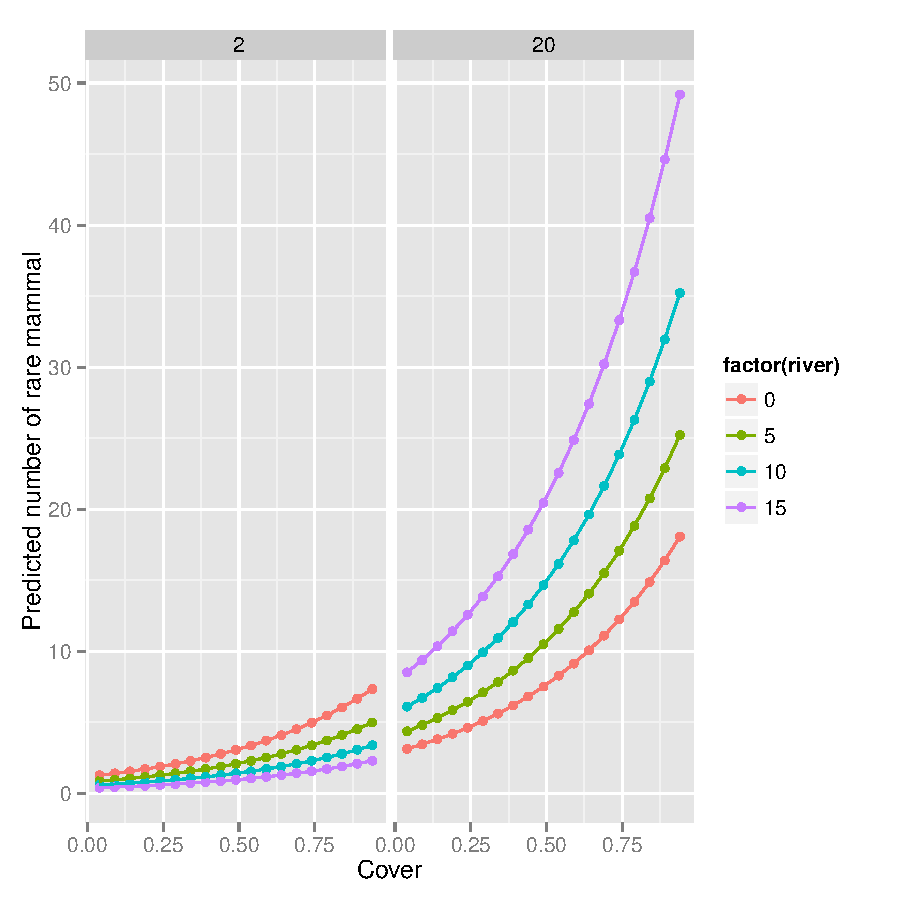
\includegraphics{HW07PLS206F14-012}







\end{document}
